\section{Modellazione dei protocolli mediante UML}
%•  Object diagram e sequence diagram (pro e contro nell'utilizzo per la modellazione di protocolli e perchè nel nostro caso possiamo considerarli equivalenti)

%Un protocollo è un insieme di regole e linee guida per la comunicazione tra due o più agenti.\\
Per la modellazione dei protocolli \footnote{per protocolli si intendono protocolli di sicurezza come Needham Schroeder Symmetric Key, protocolli di comunicazione come ARP e protocolli di encryption come RSA} si è deciso di utilizzare lo standard UML (Unified Modeling Language) nella versione 2.4\footnote{\url{https://www.omg.org/spec/UML/2.4/About-UML/}}, questo perchè questo tipo di modellazione ha una notazione semi-grafica che consente al progettista di ragionare semplicemente sulla logica del protocollo, senza dover porre eccessiva attenzione a come effettivamente deve essere implementato e senza dover necessariamente scrivere codice per la sua rappresentazione.\\  
Un modello UML è composto da un insieme di diagrammi correlati tra loro ed ogni diagramma è costituito da diversi elementi.\\
Esistono 14 tipi di diagrammi nella modellazione UML, suddivisi in diagrammi strutturali e diagrammi comportamentali (o di interazione).\\ 
Tra i vari tipi di diagrammi il più adatto alla rappresentazione dei protocolli è il sequence diagram, un diagramma comportamentale, definito per la rappresentazione dettagliata delle interazioni tra gli agenti (componenti hardware o software) partecipanti al protocollo.\\
Una caratteristica di questo tipo di diagramma è che nell'asse verticale viene rappresentato il tempo, quindi è possibile rappresentare in ordine le interazioni degli agenti dall'alto verso il basso.\\
%in ordine cronologico, infatti il tempo viene rappresentato sull'asse verticale del diagramma.\\
In alternativa può essere utilizzato l'object diagram, un diagramma di tipo strutturale nel quale vengono rappresentate le relazioni tra i vari oggetti che compongono il sistema, nel nostro caso le relazioni e gli oggetti corrispondono rispettivamente a interazioni e agenti del sequence diagram.\\
Nella Sezione \ref{sub:con} verrà spiegato in dettaglio perchè si può utilizzare indifferentemente uno tra questi due tipi di diagrammi.\\

%ma, per la rappresentazione di protocolli, si è scelto di utilizzare i sequence diagram oppure l'object diagram perchè il sequence diagram è stato definito per la rappresentazione della comunicazione \\

%Il sequence diagram è un tipo di diagramma comportamentale utilizzato per rappresentare in dettaglio le varie interazioni tra gli agenti che collaborano, la peculiarità di questo diagramma è quella di essere in grado di rappresentare uno scenario in relazione al tempo, infatti il tempo viene rappresentato sull'asse verticale del diagramma, mentre l'object diagram è un tipo di diagramma strutturale nel quale vengono rappresentate le relazioni tra i vari oggetti che compongono il sistema.


%Un modello UML è composto da un insieme di diagrammi correlati tra loro.\\
%In ogni diagramma troviamo elementi grafici dal significato formale ben definito\fixnote{mr}{siamo sicuri?}, elementi testuali formali ed elementi di testo libero.\\
%Esistono vari tipi di diagrammi nella modellazione UML, quelli che più si adattano al nostro obiettivo sono i sequence diagram e gli object diagram\fixnote{mr}{perch\'e?}.\\
%Il sequence diagram è un tipo di diagramma utilizzato per rappresentare in dettaglio le varie interazioni tra gli agenti che collaborano, la peculiarità di questo diagramma è quella di essere in grado di rappresentare uno scenario in relazione al tempo, infatti il tempo viene rappresentato sull'asse verticale del diagramma, mentre l'object diagram è un tipo di diagramma statico nel quale vengono rappresentate le relazioni tra i vari oggetti che compongono il sistema.

\subsection{Confronto tra sequence diagram e object diagram}\label{sub:con}

Per la modellazione tramite lo standard UML è stato utilizzato il tool, open source, Modelio nella versione 4.1.\\
Dato il il protocollo Needham Schroeder Symmetric Key descritto in \cite{NS78}:
\begin{lstlisting}[mathescape]
    1. $A \rightarrow S : A, B, N_a$
    2. $S \rightarrow A : \{N_a, K_{ab}, B, \{K_{ab}, A\}_{K_{bs}}\}_{K_{as}}$
    3. $A \rightarrow B : \{K_{ab}, A\}_{K_{bs}}$
    4. $B \rightarrow A : \{N_b\}_{K_{as}}$
    5. $A \rightarrow B : \{N_b-1\}_{K_{as}}$
\end{lstlisting}
Le figure \ref*{fig:sd}-\ref*{fig:od}, rappresentano l'interazione tra l'agente A e l'agente B nel punto 3 del protocollo rispettivamente con un sequence ed un object diagram.\\
Più precisamente vegono rappresentate le operazioni fatte dall'agente A una volta ricevuta la chiave simmetrica da utilizzare con B dal server S.\\
Si può notare come l'agente A decifra con la chiave condivisa con il server S il pacchetto, ed inoltra all'agente B il pacchetto cifrato con la chiave condivisa tra B e S, contenente la chiave simmetrica tra A e B.\\

%Nelle figure \ref*{fig:sd}-\ref*{fig:od} è rappresentato il protocollo Needham Schroeder Symmetric Key \cite{NS78}, sia con un object diagram [Figura \ref*{fig:od}]. \\
%\fixnote{mr}{il protocollo Needham Schroeder Symmetric Key [referenza]}, sia con un sequence diagram [Figura \ref*{fig:sd}], sia con un object diagram [Figura \ref*{fig:od}]. \\
%In particolare questo esempio consiste nel primo messaggio inviato dall'agente Initiator, che vuole iniziare una comunicazione con l'agente Recipient, contenente la chiave simmetrica e l'identità dell'agente Initiator, il tutto cifrato con la chiave simmetrica condivisa tra il server S e l'agente Recipient.\fixnote{mr}{di solito io metto dei numeri sui messaggi nella figura e poi li uso nel testo per non far perdere il lettore}\\
%\fixnote{mr}{meglio mettere gli agenti A e B come lifeline, o cambiare il modo con cui ci riferiamo agli agenti nel testo}, che vuole iniziare una comunicazione con l'agente B\fixnote{mr}{di solito io metto dei numeri sui messaggi nella figura e poi li uso nel testo per non far perdere il lettore}, contenente la chiave simmetrica e l'identità dell'agente A, il tutto cifrato con la chiave simmetrica condivisa tra il server S e l'agente B.
\begin{figure}[h!] 
    \centering 
        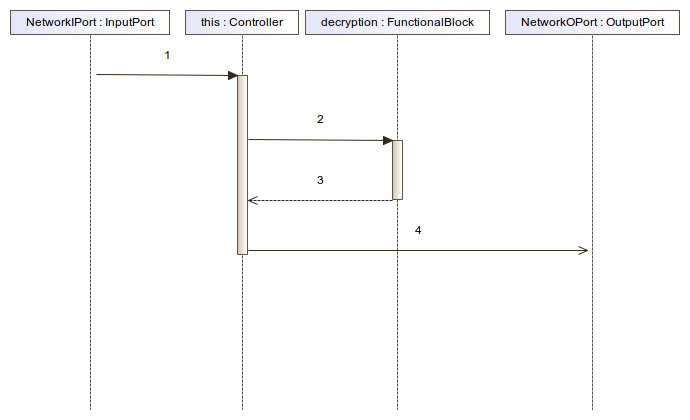
\includegraphics[width=\textwidth]{img/FirstMessage.png} 
        \caption{Sequence diagram: Inoltro pacchetto da A a B} 
        \label{fig:sd}
\end{figure}
\newpage
\begin{figure}[h!]
    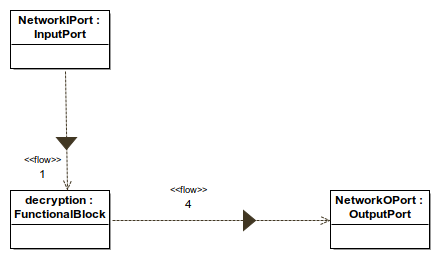
\includegraphics[scale=0.8]{img/FirstMessage_2.png} 
    \caption{Object diagram: Inoltro pacchetto da A a B} 
    \label{fig:od}
\end{figure}

\begin{lstlisting}[frame=single, mathescape, basicstyle=\footnotesize]
1. $<\{A.nonce, B.name, SK(A,B), \{A.name,SK(A,B)\}\_SK(B,S)\}\_SK(A,S)>$
2. $<\{A.nonce, B.name, SK(A,B), \{A.name,SK(A,B)\}\_SK(B,S)\}\_SK(A,S)>$
3. $<\{A.nonce, B.name, SK(A,B), \{A.name,SK(A,B)\}\_SK(B,S)\}>$
4. $<\{A.name,SK(A,B)\}\_SK(B,S)\}>$
\end{lstlisting}
% \begin{enumerate}
% \item $\{i.nonce, r,name, SymKey(i,r), \{i.name,SymKey(i,r)\}\_SharedKey(r,s)\}\_SharedKey(i,s)$
% \item $<\{i.nonce, r,name, SymKey(i,r), \{i.name,SymKey(i,r)\}\_SharedKey(r,s)\}\_SharedKey(i,s)>$
% \item $\{i.nonce, r,name, SymKey(i,r), \{i.name,SymKey(i,r)\}\_SharedKey(r,s)\}$
% \item $\{i.name,SymKey(i,r)\}\_SharedKey(r,s)\}$
% \end{enumerate}


% \begin{figure}[h!] 
%     \centering 
%     \subfloat[Sequence diagram]{
%         \includegraphics[width=\textwidth]{img/NSSK/Sequencediagram/FirstMessage.png} 
%         \label{fig:sd}
%     }
%     \subfloat[Object diagram]{
%         \includegraphics[width=\textwidth]{img/NSSK/Objectdiagram/FirstMessage.png} 
%         \label{fig:od}
    
%     }
%     \caption{Inoltro pacchetto da A a B} 
%     \label{fig:exampleOvsS}
% \end{figure}

\noindent Come possiamo vedere, nei due tipi di diagramma viene rappresentata sia la modellazione della parte fisica che andrà ad utilizzare il protocollo, sia la modellazione della parte logica sul funzionamento del protocollo.\\
La modellazione fisica è rappresentata dagli elementi di tipo InputPort ed OutputPort, i quali sono gli unici elementi fisici nei diagrammi utilizzati come punto di contatto tra i modelli del software e dell'hardware, e guardando le lifelines in Figura \ref*{fig:sd} si può notare anche il Controller, il quale è il dispositivo proprietario delle porte.\\
Gli elementi di tipo FunctionalBlock fanno parte della rappresentazione della modellazione logica del protocollo, vengono utilizzati per la codifica di un'operazione che non può essere dettagliata maggiormente (oppure non è necessario farlo considerando l'obiettivo della verifica di questo modello) che, presi degli input, restituisce un output.\\
Nel caso in cui si voglia rappresentare un insieme di operazioni si utilizzano gli elementi di tipo FunctionalArchitecture, questi vengono utilizzati come "segnaposto" per l'insieme di operazioni che verrà descritto in un altro diagramma.\\  
In entrambi i diagrammi le information flow rappresentano gli input e gli output dei vari elementi, nelle etichette vengono descritti i parametri passati, per convenzione se i parametri si trovano tra \{ \} significa che l'input o l'output di un oggetto è un pacchetto.\\
Modelio consente di esportare i modelli UML in file .xmi (XML Metadata Interchange), uno standard basato sulla struttura XML che ne consente lo scambio tra applicazioni.\\
%Nel file .xmi ogni blocco (o lifeline) viene identificato tramite un codice univoco (id) e ne vengono descritte tutte le proprietà, anche le frecce etichettate con i parametri vengono identificate tramite un id e gli id dei blocchi vengono utilizzati per indicare il blocco di partenza e quello d'arrivo, le informazioni riportate sull'etichetta della freccia vengono inserite tra le sue proprietà.
Nel file .xmi, strutturato come un xml, troviamo i tag per l'identificazione tramite codice univoco (id) degli elementi (lifelines, oggetti, information flow) e i tag per descrivere le proprietà dei vari elementi (tipo, nome, descrizione).\\
Tra le proprietà degli elementi di tipo information flow (frecce) sono presenti i tag per identificare tramite id l'elemento sorgente e l'elemento destinazione delle informazioni.\\
Analizzando il file .xmi estratto da un protocollo modellato tramite sequence diagram o da un protocollo modellato tramite object diagram, possiamo vedere come l'estrazione delle lifelines del sequence diagram corrisponde all'estrazione degli oggetti dell'object diagram e l'estrazione delle information flow viene rappresentata nello stesso modo.\\
Questo ci consente di affermare che utilizzando uno a scelta tra i due diagrammi è possibile modellare un protocollo senza la perdita di alcuna informazione.\\
%L'ordine delle interazioni descritte dal sequence diagram viene preservato nell'object diagram seguendo l'orientamento delle information flow dal primo oggetto.\\
%\fixnote{mr}{credo debba essere giustificato. di solito l'espressivit\`a \`e uguale se si possono dimostrare le stesse propriet\`a. Magari in questo cosa possiamo dire che riusciamo ad esprimere gli stessi concetti - ma dobbiamo dare chiarezza sul perch\'e sono effettivamente gli stessi concetti} che il grado di espressività dei due diagrammi è il medesimo, ed è proprio per questo motivo che ai fini dei nostri obiettivi è indifferente utilizzare uno tra questi due tipi di diagrammi per la modellazione di un protocollo.\\
Il file .xmi può essere utilizzato come input di un software in grado di navigarne la struttura e restituire in output dei file pronti per essere utilizzati dai tool di verifica formale dei protocolli, ad esempio il software potrebbe restituire come output un file scritto in Applied Pi Calcus pronto per essere utilizzato come input dal tool ProVerif (Sezione \ref*{sub:pro}).
%\'E possibile utilizzare il file .xmi come input per un software in grado di navigarne la struttura e generare un file di output scritto in un qualsiasi\fixnote{toglierei qualsiasi e direi w.r.t. i lang che abbiamo considerato} linguaggio utilizzato dai tool per la verifica formale di protocolli.
%Dal file .xmi è possibile creare un software in grado navigarne la struttura e generare un file di output in un linguaggio utilizzato da un tool per la verifica formale di protocolli. 

% \lstset{
%   basicstyle=\ttfamily,
%   showstringspaces=false,
%   commentstyle=\color{gray}\upshape
% }
\newpage
\begin{figure}[h!]
    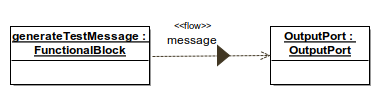
\includegraphics[scale=0.7]{xmi/ex.png} 
    \caption{Esempio di modellazione con object diagram}
\end{figure}

\begin{figure} [h!]
    \lstinputlisting[language=XMI, breaklines= true]{xmi/ex.xmi}
    \caption{Esempio di estreazione di un file .xmi}
\end{figure}

\newpage
%\noindent Per completezza in appendice \ref*{appendix:a} si può trovare la modellazione completa del protocollo di Needham-Schroeder a chiave simmetrica, oltre alla modellazione del protocollo ARP e di RSA.





